\documentclass[border=3pt]{standalone}
% Preâmbulo compartilhado pelos diagramas TikZ da aula 7 de Navegação (Implementação do A*)
\usepackage[T1]{fontenc}
\usepackage[utf8]{inputenc}
\usepackage{lmodern}
\usepackage{amsmath}
\usepackage{xcolor}
\usepackage{tikz}
\usetikzlibrary{arrows.meta,angles,quotes,decorations.pathmorphing,decorations.pathreplacing,calc,
                positioning,shapes.geometric,shapes.misc,backgrounds,fit,
                math}

% Paleta (mesma dos SVGs originais)
\definecolor{dblue}{HTML}{2A5B8C}
\definecolor{dorange}{HTML}{B3541E}
\definecolor{dgreen}{HTML}{4A7C59}
\definecolor{dred}{HTML}{9C4B4B}
\definecolor{dcream}{HTML}{F4F1EA}
\definecolor{dshade}{HTML}{DDD7C9}

% Função gaussiana (não normalizada por padrão de escala visual)
\pgfmathdeclarefunction{gauss}{3}{%
  \pgfmathparse{1/(#3*sqrt(2*pi))*exp(-((#1-#2)^2)/(2*#3^2))}%
}

% Estilos comuns (prefixo d... para não colidir com chaves internas do pgf)
\tikzset{
  >={Stealth[length=2mm]},
  dguide/.style={gray!55, dashed, line width=0.4pt},
  daxis/.style={gray!60, line width=0.7pt, ->},
  dbody/.style={fill=black!3, draw=black!80, line width=1pt},
  dacc/.style={draw=dblue, line width=1pt},
  dlbl/.style={black!55, font=\small},
  dsub/.style={black!45, font=\footnotesize},
  dstate/.style={circle, draw=black!80, fill=dcream, line width=1pt,
                 minimum size=17mm, font=\large, inner sep=1pt},
  dobs/.style={circle, draw=black!80, fill=dshade, line width=1pt,
               minimum size=14mm, font=\large, inner sep=1pt},
  dbox/.style={rounded corners=2pt, draw=black!80, fill=dcream, line width=1pt,
               align=center, inner sep=6pt},
  dop/.style={circle, draw=black!80, fill=white, line width=1pt,
              minimum size=6mm, inner sep=0pt, font=\small},
  dtrans/.style={->, dblue, line width=1pt},
  dmeas/.style={->, dorange, line width=1pt},
  dcurve/.style={line width=1pt, dblue},
  dcurveb/.style={line width=1.4pt, dorange},
}

\begin{document}
\hyphenpenalty=10000 \exhyphenpenalty=10000 \tolerance=9999 \emergencystretch=3em
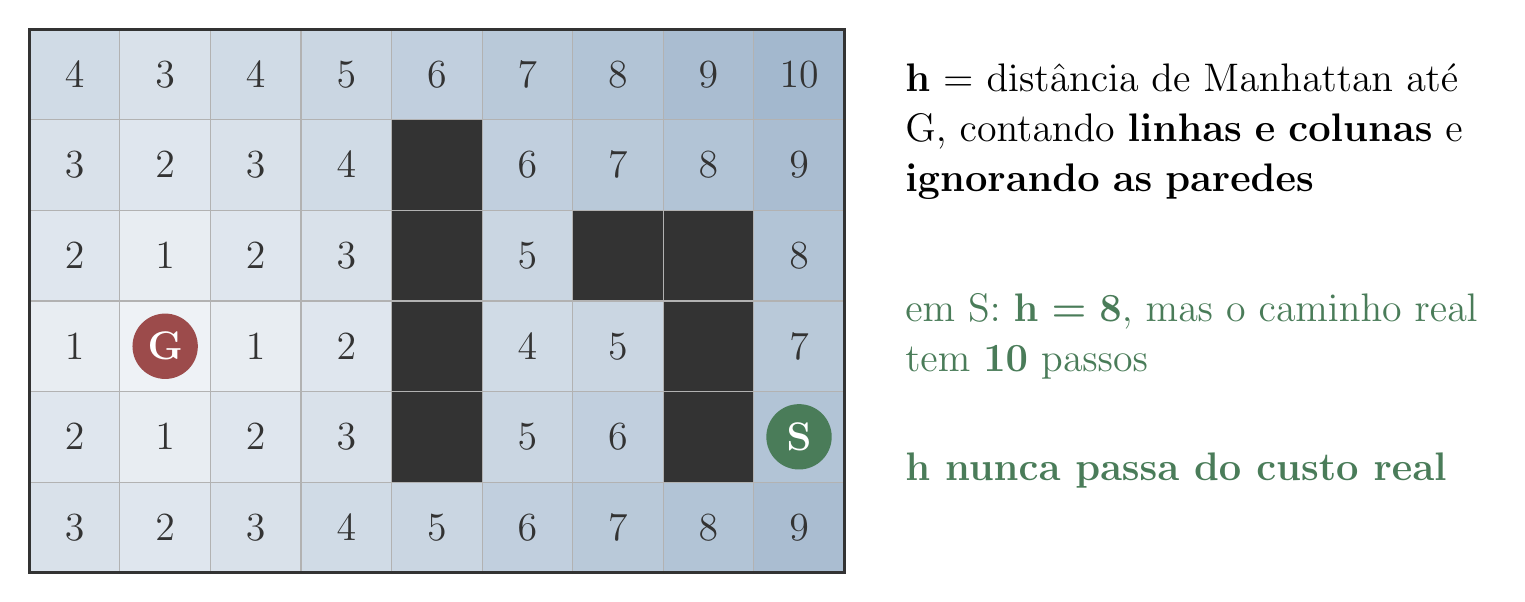
\begin{tikzpicture}[x=1cm,y=1cm]
\draw[fill=dblue!22!white, draw=black!30, line width=0.4pt] (0.000,5.750) rectangle ++(1.150,1.150);
\draw[fill=dblue!18!white, draw=black!30, line width=0.4pt] (1.150,5.750) rectangle ++(1.150,1.150);
\draw[fill=dblue!22!white, draw=black!30, line width=0.4pt] (2.300,5.750) rectangle ++(1.150,1.150);
\draw[fill=dblue!25!white, draw=black!30, line width=0.4pt] (3.450,5.750) rectangle ++(1.150,1.150);
\draw[fill=dblue!29!white, draw=black!30, line width=0.4pt] (4.600,5.750) rectangle ++(1.150,1.150);
\draw[fill=dblue!33!white, draw=black!30, line width=0.4pt] (5.750,5.750) rectangle ++(1.150,1.150);
\draw[fill=dblue!36!white, draw=black!30, line width=0.4pt] (6.900,5.750) rectangle ++(1.150,1.150);
\draw[fill=dblue!40!white, draw=black!30, line width=0.4pt] (8.050,5.750) rectangle ++(1.150,1.150);
\draw[fill=dblue!43!white, draw=black!30, line width=0.4pt] (9.200,5.750) rectangle ++(1.150,1.150);
\draw[fill=dblue!18!white, draw=black!30, line width=0.4pt] (0.000,4.600) rectangle ++(1.150,1.150);
\draw[fill=dblue!15!white, draw=black!30, line width=0.4pt] (1.150,4.600) rectangle ++(1.150,1.150);
\draw[fill=dblue!18!white, draw=black!30, line width=0.4pt] (2.300,4.600) rectangle ++(1.150,1.150);
\draw[fill=dblue!22!white, draw=black!30, line width=0.4pt] (3.450,4.600) rectangle ++(1.150,1.150);
\draw[fill=black!80, draw=black!30, line width=0.4pt] (4.600,4.600) rectangle ++(1.150,1.150);
\draw[fill=dblue!29!white, draw=black!30, line width=0.4pt] (5.750,4.600) rectangle ++(1.150,1.150);
\draw[fill=dblue!33!white, draw=black!30, line width=0.4pt] (6.900,4.600) rectangle ++(1.150,1.150);
\draw[fill=dblue!36!white, draw=black!30, line width=0.4pt] (8.050,4.600) rectangle ++(1.150,1.150);
\draw[fill=dblue!40!white, draw=black!30, line width=0.4pt] (9.200,4.600) rectangle ++(1.150,1.150);
\draw[fill=dblue!15!white, draw=black!30, line width=0.4pt] (0.000,3.450) rectangle ++(1.150,1.150);
\draw[fill=dblue!11!white, draw=black!30, line width=0.4pt] (1.150,3.450) rectangle ++(1.150,1.150);
\draw[fill=dblue!15!white, draw=black!30, line width=0.4pt] (2.300,3.450) rectangle ++(1.150,1.150);
\draw[fill=dblue!18!white, draw=black!30, line width=0.4pt] (3.450,3.450) rectangle ++(1.150,1.150);
\draw[fill=black!80, draw=black!30, line width=0.4pt] (4.600,3.450) rectangle ++(1.150,1.150);
\draw[fill=dblue!25!white, draw=black!30, line width=0.4pt] (5.750,3.450) rectangle ++(1.150,1.150);
\draw[fill=black!80, draw=black!30, line width=0.4pt] (6.900,3.450) rectangle ++(1.150,1.150);
\draw[fill=black!80, draw=black!30, line width=0.4pt] (8.050,3.450) rectangle ++(1.150,1.150);
\draw[fill=dblue!36!white, draw=black!30, line width=0.4pt] (9.200,3.450) rectangle ++(1.150,1.150);
\draw[fill=dblue!11!white, draw=black!30, line width=0.4pt] (0.000,2.300) rectangle ++(1.150,1.150);
\draw[fill=dblue!8!white, draw=black!30, line width=0.4pt] (1.150,2.300) rectangle ++(1.150,1.150);
\draw[fill=dblue!11!white, draw=black!30, line width=0.4pt] (2.300,2.300) rectangle ++(1.150,1.150);
\draw[fill=dblue!15!white, draw=black!30, line width=0.4pt] (3.450,2.300) rectangle ++(1.150,1.150);
\draw[fill=black!80, draw=black!30, line width=0.4pt] (4.600,2.300) rectangle ++(1.150,1.150);
\draw[fill=dblue!22!white, draw=black!30, line width=0.4pt] (5.750,2.300) rectangle ++(1.150,1.150);
\draw[fill=dblue!25!white, draw=black!30, line width=0.4pt] (6.900,2.300) rectangle ++(1.150,1.150);
\draw[fill=black!80, draw=black!30, line width=0.4pt] (8.050,2.300) rectangle ++(1.150,1.150);
\draw[fill=dblue!33!white, draw=black!30, line width=0.4pt] (9.200,2.300) rectangle ++(1.150,1.150);
\draw[fill=dblue!15!white, draw=black!30, line width=0.4pt] (0.000,1.150) rectangle ++(1.150,1.150);
\draw[fill=dblue!11!white, draw=black!30, line width=0.4pt] (1.150,1.150) rectangle ++(1.150,1.150);
\draw[fill=dblue!15!white, draw=black!30, line width=0.4pt] (2.300,1.150) rectangle ++(1.150,1.150);
\draw[fill=dblue!18!white, draw=black!30, line width=0.4pt] (3.450,1.150) rectangle ++(1.150,1.150);
\draw[fill=black!80, draw=black!30, line width=0.4pt] (4.600,1.150) rectangle ++(1.150,1.150);
\draw[fill=dblue!25!white, draw=black!30, line width=0.4pt] (5.750,1.150) rectangle ++(1.150,1.150);
\draw[fill=dblue!29!white, draw=black!30, line width=0.4pt] (6.900,1.150) rectangle ++(1.150,1.150);
\draw[fill=black!80, draw=black!30, line width=0.4pt] (8.050,1.150) rectangle ++(1.150,1.150);
\draw[fill=dblue!36!white, draw=black!30, line width=0.4pt] (9.200,1.150) rectangle ++(1.150,1.150);
\draw[fill=dblue!18!white, draw=black!30, line width=0.4pt] (0.000,0.000) rectangle ++(1.150,1.150);
\draw[fill=dblue!15!white, draw=black!30, line width=0.4pt] (1.150,0.000) rectangle ++(1.150,1.150);
\draw[fill=dblue!18!white, draw=black!30, line width=0.4pt] (2.300,0.000) rectangle ++(1.150,1.150);
\draw[fill=dblue!22!white, draw=black!30, line width=0.4pt] (3.450,0.000) rectangle ++(1.150,1.150);
\draw[fill=dblue!25!white, draw=black!30, line width=0.4pt] (4.600,0.000) rectangle ++(1.150,1.150);
\draw[fill=dblue!29!white, draw=black!30, line width=0.4pt] (5.750,0.000) rectangle ++(1.150,1.150);
\draw[fill=dblue!33!white, draw=black!30, line width=0.4pt] (6.900,0.000) rectangle ++(1.150,1.150);
\draw[fill=dblue!36!white, draw=black!30, line width=0.4pt] (8.050,0.000) rectangle ++(1.150,1.150);
\draw[fill=dblue!40!white, draw=black!30, line width=0.4pt] (9.200,0.000) rectangle ++(1.150,1.150);
\draw[black!80, line width=1.2pt] (0.000,0.000) rectangle (10.350,6.900);
\node[font=\Large, black!80] at (0.575,6.325) {4};
\node[font=\Large, black!80] at (1.725,6.325) {3};
\node[font=\Large, black!80] at (2.875,6.325) {4};
\node[font=\Large, black!80] at (4.025,6.325) {5};
\node[font=\Large, black!80] at (5.175,6.325) {6};
\node[font=\Large, black!80] at (6.325,6.325) {7};
\node[font=\Large, black!80] at (7.475,6.325) {8};
\node[font=\Large, black!80] at (8.625,6.325) {9};
\node[font=\Large, black!80] at (9.775,6.325) {10};
\node[font=\Large, black!80] at (0.575,5.175) {3};
\node[font=\Large, black!80] at (1.725,5.175) {2};
\node[font=\Large, black!80] at (2.875,5.175) {3};
\node[font=\Large, black!80] at (4.025,5.175) {4};
\node[font=\Large, black!80] at (6.325,5.175) {6};
\node[font=\Large, black!80] at (7.475,5.175) {7};
\node[font=\Large, black!80] at (8.625,5.175) {8};
\node[font=\Large, black!80] at (9.775,5.175) {9};
\node[font=\Large, black!80] at (0.575,4.025) {2};
\node[font=\Large, black!80] at (1.725,4.025) {1};
\node[font=\Large, black!80] at (2.875,4.025) {2};
\node[font=\Large, black!80] at (4.025,4.025) {3};
\node[font=\Large, black!80] at (6.325,4.025) {5};
\node[font=\Large, black!80] at (9.775,4.025) {8};
\node[font=\Large, black!80] at (0.575,2.875) {1};
\node[font=\Large, black!80] at (1.725,2.875) {0};
\node[font=\Large, black!80] at (2.875,2.875) {1};
\node[font=\Large, black!80] at (4.025,2.875) {2};
\node[font=\Large, black!80] at (6.325,2.875) {4};
\node[font=\Large, black!80] at (7.475,2.875) {5};
\node[font=\Large, black!80] at (9.775,2.875) {7};
\node[font=\Large, black!80] at (0.575,1.725) {2};
\node[font=\Large, black!80] at (1.725,1.725) {1};
\node[font=\Large, black!80] at (2.875,1.725) {2};
\node[font=\Large, black!80] at (4.025,1.725) {3};
\node[font=\Large, black!80] at (6.325,1.725) {5};
\node[font=\Large, black!80] at (7.475,1.725) {6};
\node[font=\Large, black!80] at (9.775,1.725) {8};
\node[font=\Large, black!80] at (0.575,0.575) {3};
\node[font=\Large, black!80] at (1.725,0.575) {2};
\node[font=\Large, black!80] at (2.875,0.575) {3};
\node[font=\Large, black!80] at (4.025,0.575) {4};
\node[font=\Large, black!80] at (5.175,0.575) {5};
\node[font=\Large, black!80] at (6.325,0.575) {6};
\node[font=\Large, black!80] at (7.475,0.575) {7};
\node[font=\Large, black!80] at (8.625,0.575) {8};
\node[font=\Large, black!80] at (9.775,0.575) {9};
\node[circle, fill=dgreen, text=white, font=\bfseries\Large, inner sep=1pt, minimum size=0.83cm] at (9.775,1.725) {S};
\node[circle, fill=dred, text=white, font=\bfseries\Large, inner sep=1pt, minimum size=0.83cm] at (1.725,2.875) {G};
\node[font=\Large, anchor=west, text width=7.4cm] at (11.0,5.6) {\textbf{h} = distância de Manhattan até G, contando \textbf{linhas e colunas} e \textbf{ignorando as paredes}};
\node[font=\Large, dgreen, anchor=west, text width=7.4cm] at (11.0,3.0) {em S: \textbf{h = 8}, mas o caminho real tem \textbf{10} passos};
\node[font=\Large\bfseries, dgreen, anchor=west, text width=7.4cm] at (11.0,1.3) {h nunca passa do custo real};
\end{tikzpicture}
\end{document}
